%
% FIX THIS -- remove/change, just some examples of things
%
\chapter{Computation}

\section{Game-theoretic goal recognition model}

With the game defined, the next step is computing a solution to the game. 
Before defining rational behavior, we first need to discuss the set of strategies. In a sequential game, 
a pure strategy of a player is a deterministic mapping from the
current state and the player's observations/histories leading to the state, to an available action. For the adversary, such observations/histories include its own sequence 
of prior actions and its target $\theta$. 
The observer's observations/histories include 
the adversary's sequence of actions and the observer's sequence of actions.
A mixed strategy is a randomized strategy, specified by a probability distribution over the set of pure strategies.
The strategies are defined more formally in Section \ref{stochastic_games} and Definition \ref{def:bhs}.   
%For two-player zero-sum games, the standard solution concept is the max-min solution:
%$\max_x \min_y u(x,y)$, where $x$ and $y$ are the observer's and the adversary's mixed strategies, respectively,
%and $u(x,y)$ is the expected utility to the observer given mixed strategies $x$ and $y$. One can also define
%min-max solution $ \min_y\max_x u(x,y)$. 
%For zero-sum games, the max-min value, min-max value, and Nash equilibrium value all coincide~\cite{fudenberg1991game}. 

We are interested in computing the max-min solution, 
which is equivalent to the max-min value, min-max value, and Nash equilibrium value  of the game. 
For simultaneous-move games this can usually be solved by formulating a linear program. 
However, for our sequential game, each pure strategy need to prescribe an action for each possible sequence of observations leading to that state and, as a result, the sets of pure strategies are exponential for both players. 

To overcome this computational challenge, we focus on \emph{stationary strategies}, 
which are strategies that depend only on the current 
state (for the adversary, also on $\theta$) and not on the history of observations (see Definition \ref{def:ss}).
While for stochastic games with complete information, it is known that there always exist an optimal solution that consists of stationary strategies~\cite{fudenberg1991game},
 it is an open question whether the same property holds for our setting, which is an incomplete-information game.
Nevertheless, there are some heuristic reasons
that stationary strategies are at least good approximately optimal solutions: The state (i.e., adversary's location) already capture a large amount of information about the strategic intention of the adversary.

%\vspace{-\medskipamount}
%\paragraph{Formulating the Linear Program.}
%\indent We borrow notation from \cite{....} on finite-step algorithms for single controller stochastic games. 
Restricting to stationary strategies,  randomized strategies now correspond to a mapping from state to a distribution over actions. We have thus reduced the dimension of the solution space from exponential to polynomial in the size of the graph.
Furthermore, our game exhibits the single-controller property: The state transitions are controlled by the adversary only. For complete information stochastic games with a single controller, a \emph{linear programming} (LP) formulation is known~\cite{Raghavan2003}. We adapt this LP formulation to our incomplete information setting.
 
We define $V(\theta, s)$ to be a variable that represents 
the expected payoff to the observer at state $s$ and with adversary's target begin $\theta$. 
We use $P(\theta)$ to denote the prior probability 
of $\theta \in B$ being the adversary's target such that $\sum_{\theta \in B} P(\theta) = 1$. 
The observer's objective is to find a (possibly randomized) strategy 
that maximizes his expected payoff given the prior distribution over the target set $B$, 
the moves of the adversary, and the adversary's starting location. 
The following linear program computes the utility of the observer in an max-min solution
assuming both players are playing a stationary strategy. 
\begin{align}
\!\!\!\!\max_{V, \{f_i(s)\}_{i,s}} \sum_{\theta}&P(\theta)V(\theta, s_{o}) \label{eq:game_obj}\\
V(\theta, s) &\leq \sum_{i \in B} r(s, i, j, \theta)f_{i}(s) + V(\theta, j) &\forall\theta\in B,\forall s \mid s\neq \theta, \forall j\in\nu(s)\label{eq:game_incentive}\\
V(\theta, s) &= 0 \quad &\mbox{when} \,\,\, s=\theta\label{eq:game_end}\\
\sum_{i} f_{i}(s) &= 1\quad &\forall s \label{eq:game_sum}\\
f_{i}(s) &\geq 0\quad &\forall s,i\label{eq:game_nonneg}
\end{align}
In the above linear program, \eqref{eq:game_obj} is the objective of the observer. 
The $f_{i}(s)$'s represent the probability of the observer taking an action $i \in B$ given the state $s$. 
To ensure that the probability distribution is well defined at each state of the games,
\eqref{eq:game_sum} and \eqref{eq:game_nonneg} impose the standard sum-equal-to-one and non-negative conditions on the probability of playing 
each action $i \in B$. The Bellman-like inequality \eqref{eq:game_incentive}
bounds the expected value for any state using 
expected values of next states plus the expected current reward, assuming the adversary will choose
the state transition that minimizes the observer's expected utility.
Finally, \eqref{eq:game_end} specifies the base condition when the adversary has reached their destination and the game ends. 
The size of the linear program is polynomial in the size of the graph. 
%While, in theory, the game could go on forever if the adversary never reaches his target $\theta$, 
%because of the per-timestep cost of $d$, any sufficiently long path for the adversary would be 
%dominated by the strategy of taking the shortest path to $\theta$. 
%Eliminating these dominated strategies allows us to set a finite bound for the duration of the game, 
%which grows linearly in the shortest distance to the target that is furthest away.

The solution of this linear program prescribes a randomized stationary strategy $f_i(s)$ 
for the observer and, from the dual solutions, one can compute a stationary strategy for the adversary.
In more detail, the dual linear program is
\begin{align}
\min &\sum_{s}t_s\label{eq:dual_obj}\\
t_s&\geq \sum_{\theta, j}\lambda^\theta_{s,j}r(s,i,j,\theta) &\forall s,i \label{eq:dual_incentive}\\
I_{s=s_0}P(\theta)+\sum_{s' \neq \theta: s\in \nu(s')}\lambda^\theta_{s',s} &=\sum_{j\in\nu(s)}\lambda^\theta_{s,j} &\forall\theta\in B,\forall s\neq \theta\label{eq:dual_flow}\\
\lambda^\theta_{s,j}&\geq 0    &\forall \theta,s,j
\end{align}
where $I_{s=s_0}$ is the indicator that equals 1 when $s=s_0$ and 0 otherwise.
The dual variables $\lambda^\theta_{s,j}$
can be interpreted as the probability that
adversary type $\theta$ takes the edge from $s$ to $j$.
These probabilities satisfies the flow conservation constraints \eqref{eq:dual_flow}: given $\theta$, the total flow into $s$ (the left hand side) is equal to the probability that type $\theta$ visits $s$, which should equal the total flow out of $s$ (the right hand side).
The variables $t_s$ can be interpreted as the 
contribution to defender's utility from state $s$, assuming that the defender is choosing an optimal action at each state (ensured by constraint \eqref{eq:dual_incentive}). 

Given the dual solutions $\lambda^\theta_{s,j}$, 
we can compute a stationary strategy for the adversary:
let $\pi(j|\theta,s)$ be the probability that the adversary type $\theta$ chooses $j$ at state $s$.
Then for all $\theta\in B$ and $s\neq\theta$, $\pi(j|\theta,s)=
\frac{\lambda^\theta_{s,j}}{\sum_{j'\in\nu(s)}\lambda^\theta_{s,j'}}$.
It is straightforward to verify that by playing the stationary strategy $\pi$, the adversary
type $\theta$ will visit each edge $(s,j)$ with probability
$\lambda^\theta_{s,j}$.

\begin{lemma}
Given a stationary strategy for the defender, 
there exists a best response strategy for the adversary that is also a stationary strategy.
\end{lemma}
\begin{proof}[Sketch]
Given a stationary defender strategy $f_i(s)$, each adversary type $\theta$ now faces a Markov Decision Process (MDP)
problem, which admits a stationary strategy as its optimal solution.
\end{proof} 

More specifically,
since the state transitions are deterministic and fully controlled by the adversary,
each type $\theta$ faces a problem of determining the shortest path from $s_0$ to $\theta$, 
with the cost of each edge $(s,j)$ as
$\sum_{i\in B}f_i(s) r(s,i,j,\theta)$.
Looking into the components of $r(s,i,j,\theta)$, since the adversary reward $u^\theta$ for reaching target $\theta$ occurs exactly once at the target $\theta$,
it can be canceled out and the problem is equivalent to the shortest path problem from $s_0$ to $\theta$ with
edge cost $d+f_\theta(s) q$. Since edge costs are nonnegative the shortest paths will not involve cycles.

What this lemma implies is that if the defender plays the stationary strategy prescribed by the LP \eqref{eq:game_obj}, the adversary cannot 
do better than the value of the LP by deviating to a non-stationary strategy.
\begin{corollary}
If the defender plays the stationary strategy $f_i(s)$
given by the solutions of LP $\eqref{eq:game_obj}$,
the adversary's stationary strategy $\pi$ as prescribed by
LP $\eqref{eq:dual_obj}$ is a best response, i.e., no
non-stationary strategies can achieve a better outcome for the adversary.
\end{corollary}

While it is still an open question whether the defender has an optimal strategy that is stationary,
we have shown that if we restrict to  stationary strategies for the defender, it is in the best interest of the adversary to also stick to stationary strategies and our LP \eqref{eq:game_obj} do not overestimate the value of the game. 

\subsection{Game-theoretic goal recognition design model}
One can solve this GTGRD problem by brute-force, i.e., try every subset of edges to block and then for each case solve the resulting LP. The time complexity of this approach grows exponentially in $K$. 
Instead, we can encode the choice of edge removal as integer variables added to the LP formulation, resulting in a mixed-integer program (MIP). For example, we could replace
\eqref{eq:game_incentive} with
\begin{align}
V(\theta, s) \leq \sum_{i \in B} r(s, i, j, \theta)f_{i}(s) + V(\theta, j) + M z(s, j) 
\label{eq:mip_incentive}
\end{align}
where $M$ is a positive number, and 
$z(s, j)$ is a 0-1 integer variable indicating whether
the action/edge from $s$ to $j$ is blocked.
M thus represents the penalty that the attacker incurs if he nevertheless chooses to take the edge from $s$ to $j$ while it is blocked. By making $M$ sufficiently large, we can make the actions of crossing a blocked edge dominated and therefore effectively removing the edges that we block.
We also add the constraint $\sum_{s,j} z(s,j) \leq K $.
%We implemented the MIP solution utilizing off-the-shelf MIP solvers, and conduct experiments to measure its runtime performance.
%We will also explore other algorithmic approaches, including adapting ideas from existing GRD literature such as pruning techniques that we have previous proposed for GRD and S-GRD~\cite{son:16,wayllace:16}.


\subsubsection{Dual-based greedy heuristic.}
The MIP approach scales exponentially in the worst case as the size of the graph and K grows.
 We propose a heuristic method for selecting edges to block.
 We first solve the LP for goal recognition and its dual.
In particular, we look at the dual variable 
$\lambda^\theta_{s,j}$ for the constraint \eqref{eq:game_incentive}.
 This dual has the standard interpretation as the \emph{shadow price}:
it is the rate of change to the objective if we infinitesimally relax
constraint \eqref{eq:game_incentive}.

 Looking at the MIP, in particular constraint \eqref{eq:mip_incentive}, we see that by blocking off an action from $s$ to $j$ we are effectively relaxing the corresponding LP constraints \eqref{eq:game_incentive} 
indexed by $\theta,s,j$ for all $\theta\in B$.
These are the adversary's incentive constraints for going from $s$ to $j$, for all adversary types $\theta$.

Utilizing the shadow price interpretation of the duals, the sum of the duals corresponding to the 
edge from $s$ to $j$: 
$\sum_{\theta\in B} \lambda^\theta_{s,j}$
 gives the rate of change to the objective (i.e. defender's expected utility) if the edge $(s,j)$ is blocked by an infinitesimal amount.
 Choosing the edge that maximizes this,
 $\arg \max_{s,j}\sum_{\theta\in B} \lambda^\theta_{s,j}$
 we get the maximum rate of increase of our utility.
 These rates of changes hold only when the amount of relaxation (i.e., $M$) is infinitesimal. However,
 in practice we can still use this as a heuristic for choosing edges to block.\footnote{Another perspective: from the previous section we see that $\lambda^\theta_{s,j}$ is the probability that adversary type $\theta$ traverses the edge $s,j$. 
 Then if the adversary and defender do not change their strategies after the edge $(s,j)$ is blocked, the defender would receive an additional utility of 
 $M\sum_{\theta\in B} \lambda^\theta_{s,j}$ from the adversary's penalty for crossing that edge.}

When $K > 1$, we could choose the $K$ edges with the highest dual sums.
 Alternatively, we can use a greedy approach:
pick one edge  with the maximum dual sum, 
place a block on the edge and solve the updated LP for goal recognition, and pick the next edge using the updated duals, and repeat.
In our experiments, the latter greedy approach consistently achieved significantly higher expected utilities than the former.
Intuitively, by re-solving the LP after adding each edge,
we get a more accurate picture of the adversary's 
adaptations to the blocked edges.
Whereas the rates of changes used by the former approach are only accurate when the adversary do not adapt at all to the blocked edges (see footnote 1).
Our greedy heuristic is summarized as follows.
\begin{itemize} 

\item for $i=1 \ldots K$:
\begin{itemize}
\item Solve LP \eqref{eq:game_obj}, updated with the current blocked edges. If edge $(s,j)$ blocked, the corresponding constraint \eqref{eq:game_incentive} indexed $s,j,\theta$ for all $\theta$ are modified so that $M$ is added to the right hand side.
Get the primal and dual solutions.
\item Take an edge $(s^*,j^*) \in\arg \max_{s,j}\sum_{\theta\in B} \lambda^\theta_{s,j}$,
and add it to the set of blocked edges.


\end{itemize}
\item return the set of blocked edges, and the primal solution of the final LP as the defender's stationary strategy. 
\end{itemize}


\section{Experiments}
Experiments were run on a machine using OSX Yosemite version 10.10.5, with 16 GB of ram and a 2.3 GHz Intel Core i7 processor,
and were conducted on grid environments such as the one seen in Figure \ref{fig:setup}. 
In these environments, the adversary is allowed to move to adjacent nodes connected by an edge. 
$S$ denotes the starting location of the adversary while $T1$ and $T2$ denote the locations of two potential targets.
\begin{figure}[!ht]
\begin{center}
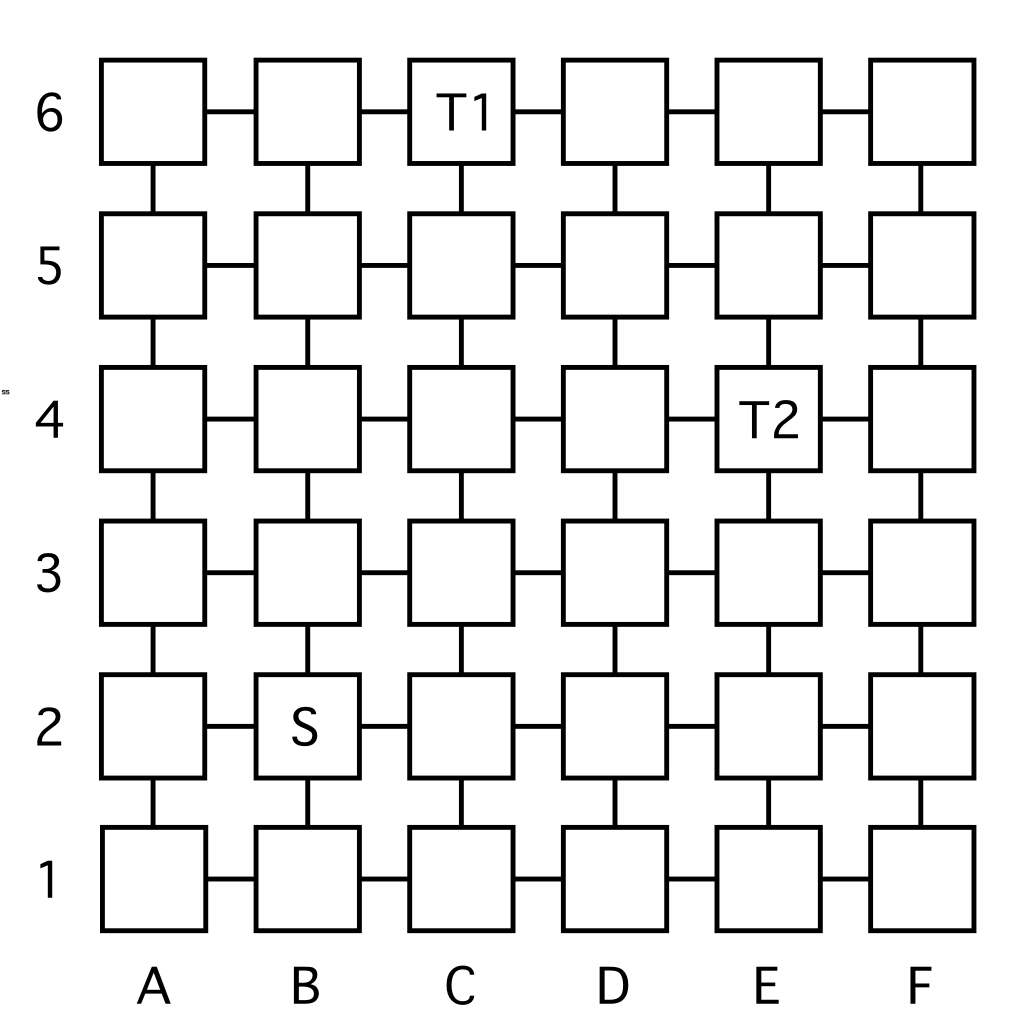
\includegraphics[width=0.4\linewidth]{graph1}
\caption{An Instance of GTGR/GTGRD Games Used in Experiments.}
\label{fig:setup}
\end{center}
\end{figure}

In Figure \ref{fig:setup}, targets $T1$ and $T2$ each have a equal likelihood of being the adversary's intended target. 
The adversary's timestep penalty $d$ and completion reward $u^{\theta}$ are both set to 0. 
The defender's reward for correctly guessing the adversary's intended target $q$ is set to $10$. 
The attacker penalty value for crossing an edge penalized by the observer is set to $10$. 
The observer is permitted to penalize 3 edges.

\subsection{A Comparison of MIP and Greedy Solutions}
As seen in Figure \ref{MIPS} and Figure \ref{GreedyS}, the mixed integer program and greedy heuristic can yield different results. 
The mixed integer program yields an expected outcome of 43.3 for the observer, 
while utilizing the greedy heuristic yields an outcome of 40.0 for the observer. 
The default expected outcome for the observer (in which no edges are penalized) is 30.0. 
The following experiments averaged the results of similar grid problems.

\begin{figure}[!ht]
\begin{center}
\begin{minipage}{0.4\linewidth}
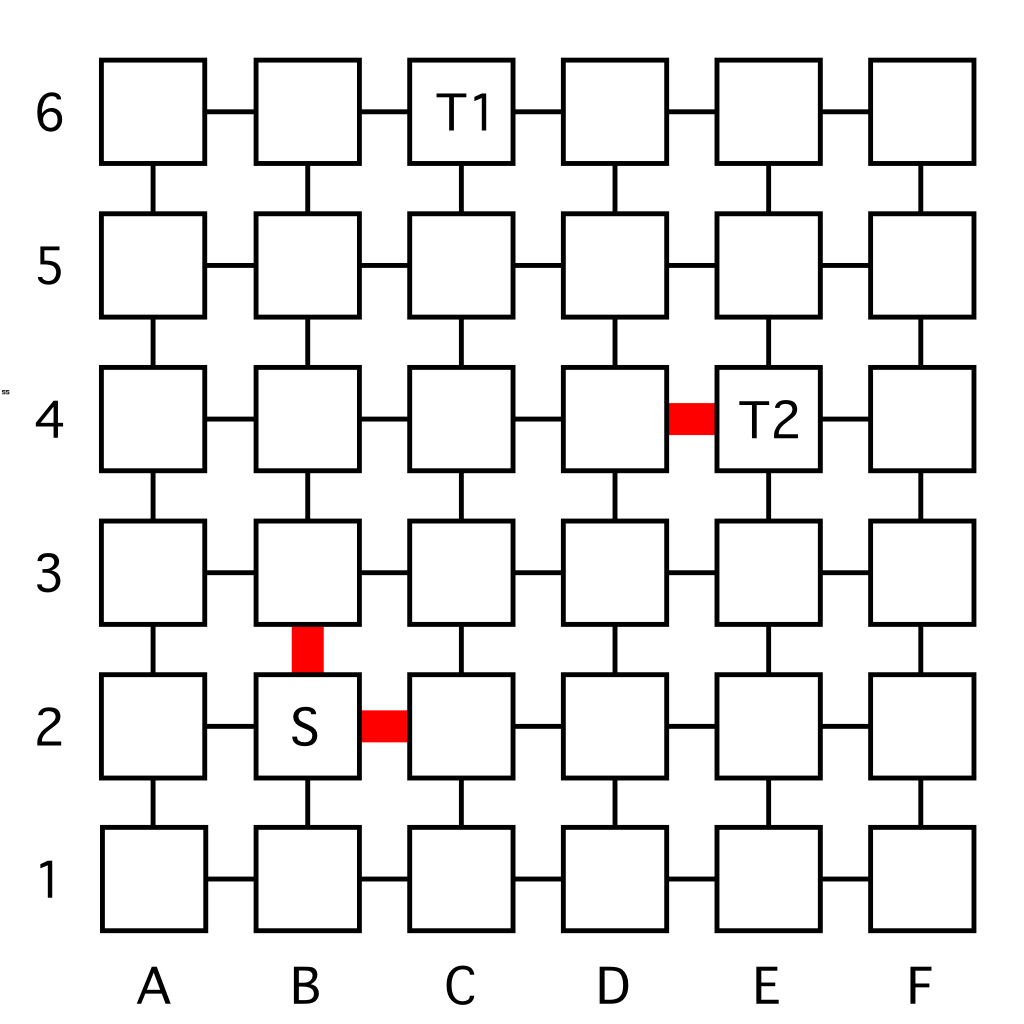
\includegraphics[width=\linewidth]{graph2}
\caption{MIP Solution}
\label{MIPS}
\end{minipage}%
\hfill
\begin{minipage}{0.4\linewidth} 
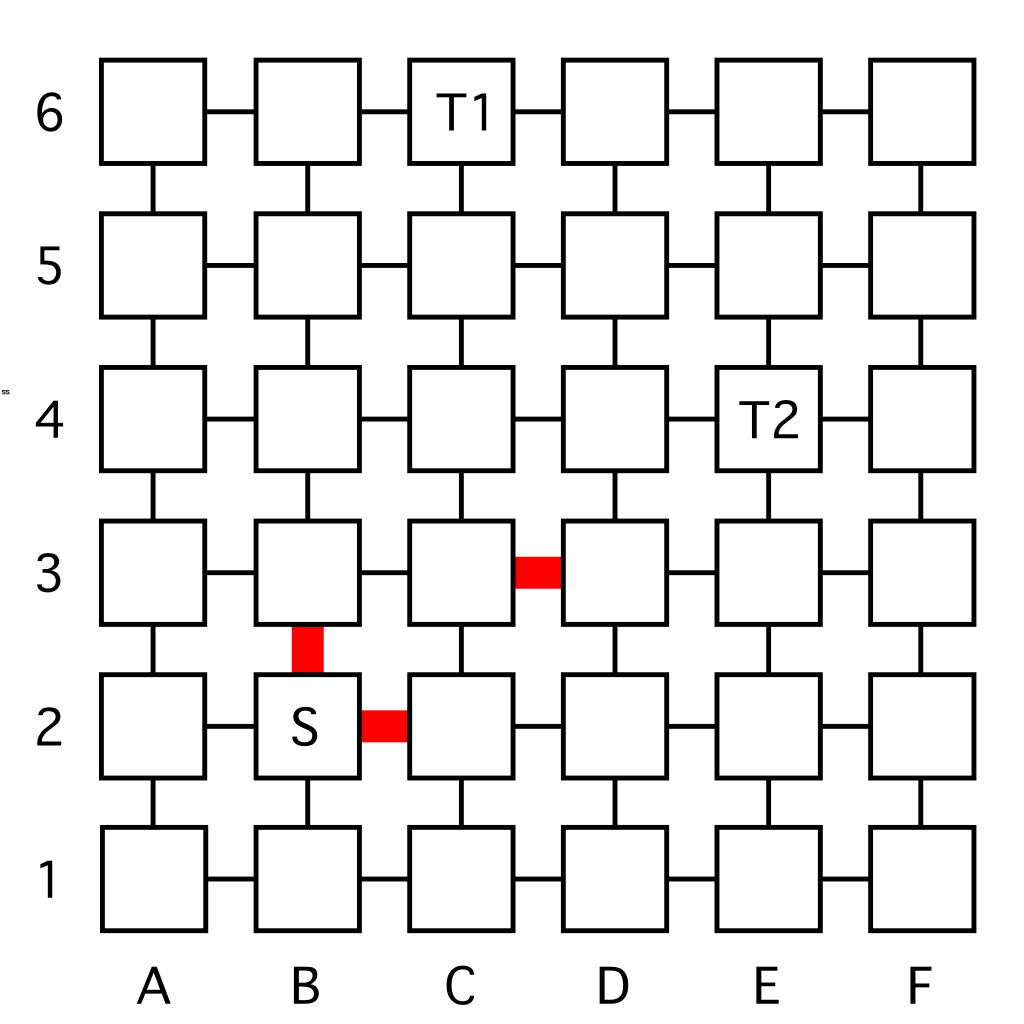
\includegraphics[width=\linewidth]{graph3}
\caption{Greedy Solution}
\label{GreedyS}
\end{minipage}
\end{center}
\end{figure}

\subsection{Running Time and Solution Quality}
Results from the following experiments were averaged over 1000 grid environments. 
For each experiment, the adversary's timestep penalty $d$ and completion reward $u^{\theta}$ were set to 0. 
For each environment, the starting location of the adversary and all targets are placed 
randomly on separate nodes. 
Additionally, each target $\theta$ is assigned a random probability $P(\theta)$ such 
that $\sum_{\theta \in B} P(\theta) = 1$. 
In all of our figures below, the greedy heuristic for the GTGRD is graphed in orange, 
the MIP is graphed in blue, 
and the default method (LP) for GTGR is graphed in grey, 
in which the game is solved with no penalized edges.
The defenders reward for correctly guessing the adversary's intended target $q$ was set to 10. 
The attacker penalty value for crossing an edge penalized by the observer was set to 10. 
Each game, the observer was permitted to penalize 2 edges.

\begin{figure}[!ht]
\begin{center}
\begin{minipage}{0.48\linewidth}
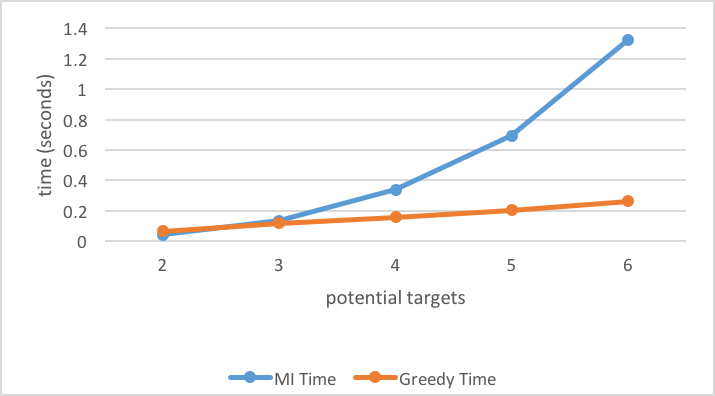
\includegraphics[width=\linewidth]{1}
\caption{Average time given targets.}
\label{fig:rt_target}
\end{minipage}%
\hfill
\begin{minipage}{0.49\linewidth}
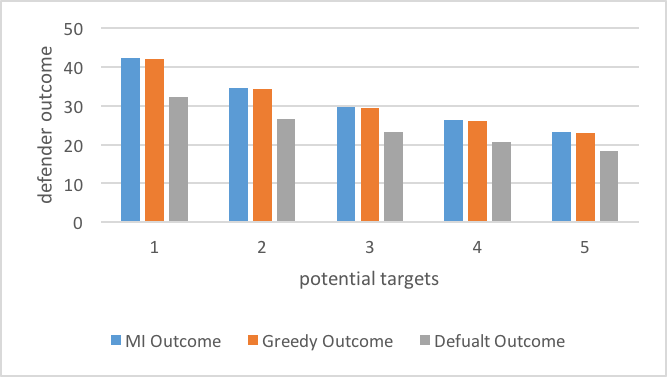
\includegraphics[width=\linewidth]{2}
\caption{Average outcome given targets.}
\label{fig:sol_target}
\end{minipage}
\end{center}
\end{figure}

\subsubsection{Various Potential Target Sizes}
In this set of experiments, we want to investigate 
the effect of different potential target sizes (i.e., $|B|$) 
to the running time (Figure \ref{fig:rt_target}) 
and solution quality (Figure \ref{fig:sol_target}) of our algorithms. 
The results are averaged over 1000 simulations of 6 by 6 grids. 
%The defender's reward for correctly guessing the adversary's intended target $q$ was set to 10. 
%The attacker penalty value for crossing an edge penalized by the observer was set to 10. 
Each game, the observer was permitted to penalize 2 edges. 

\begin{figure}[!ht]
\begin{center}
\begin{minipage}{0.48\linewidth}
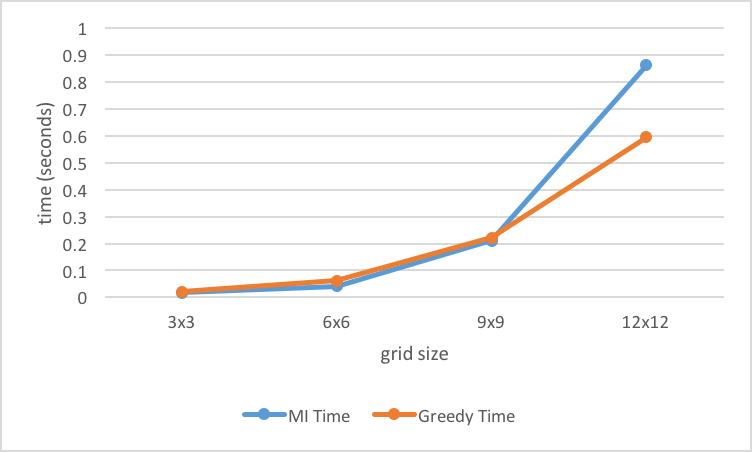
\includegraphics[width=\linewidth]{3}
\caption{Average time given size.}
\label{fig:rt_grids}
\end{minipage}%
\hfill
\begin{minipage}{0.49\linewidth}
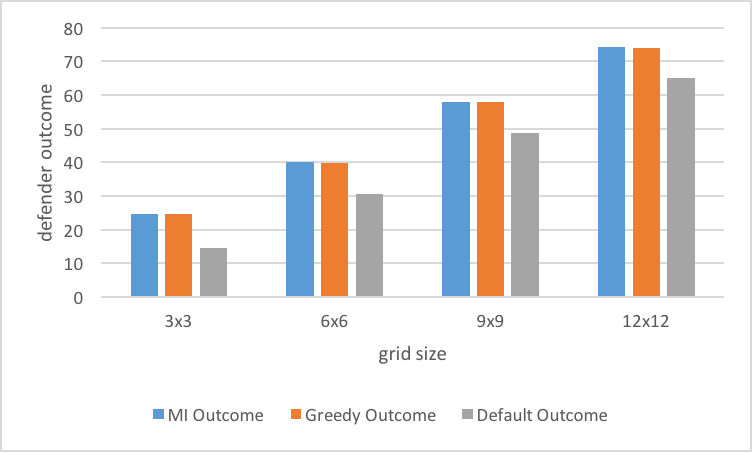
\includegraphics[width=\linewidth]{4}
\caption{Average outcome given size.}
\label{fig:sol_grids}
\end{minipage}
\end{center}
\end{figure}

As indicated in Figure \ref{fig:rt_target}, the MIP running time 
increases exponentially while the greedy heuristic running time 
remains sublinear as we increase the number of potential targets. 
Moreover, the solution quality (measured by defender's utility) 
as seen in Figure \ref{fig:sol_target} suggests that 
MIP's solution is closely aligned with our greedy heuristics. 
This gives evidence that our greedy heuristic provides good solution quality 
while achieving high efficiency. 
Note that It is no surprise that the 
defender's utility is higher in the GTGRD setting 
compared to those of GTGR. 

\subsubsection{Various Instance Sizes}
In this set of experiments, we investigate 
the effect of different instance sizes (i.e., grids) 
to the running time (Figure \ref{fig:rt_grids}) 
and solution quality (Figure \ref{fig:sol_grids}) of our algorithms. 

%Results in Figure \ref{fig:rt_grids} and Figure \ref{fig:sol_grids} are averaged over 1000 grids. 
%The defenders reward for correctly guessing the adversary's intended target $q$ was set to 10. 
%The attacker penalty value for crossing an edge penalized by the observer was set to 10. 
%Each game, the observer was permitted to penalize 2 edges.
Unlike our earlier observations on various target sizes, 
the average running times for both the MIP and our greedy heuristic 
increase significantly as we increase the instance sizes (see Figure \ref{fig:rt_grids}). 
This is not surprising as now we have more variables 
and constraints in the integer programs. 
Despite this, the defender's utilities generated by greedy heuristic are relatively 
similar to to those generated using MIP (see Figure \ref{fig:sol_grids}). 

\begin{figure}[!ht]
\begin{center}
\begin{minipage}{0.48\linewidth}
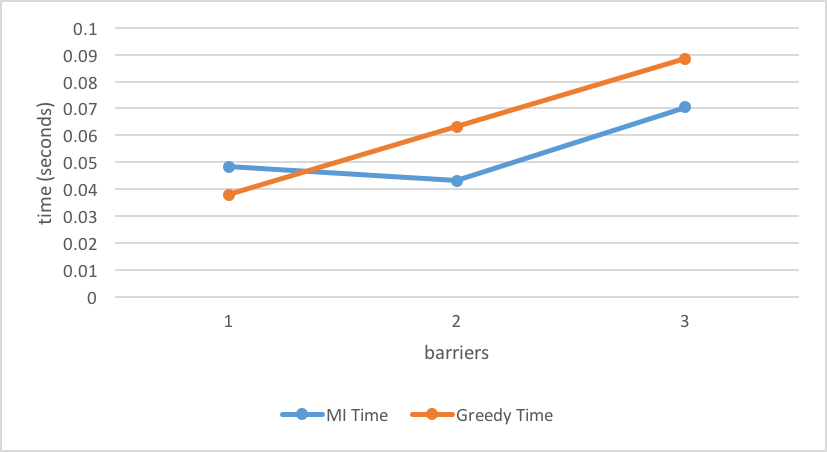
\includegraphics[width=\linewidth]{5}
\caption{Average time given penalized edges.}
\label{fig:rt_bar}
\end{minipage}%
\hfill
\begin{minipage}{0.49\linewidth}
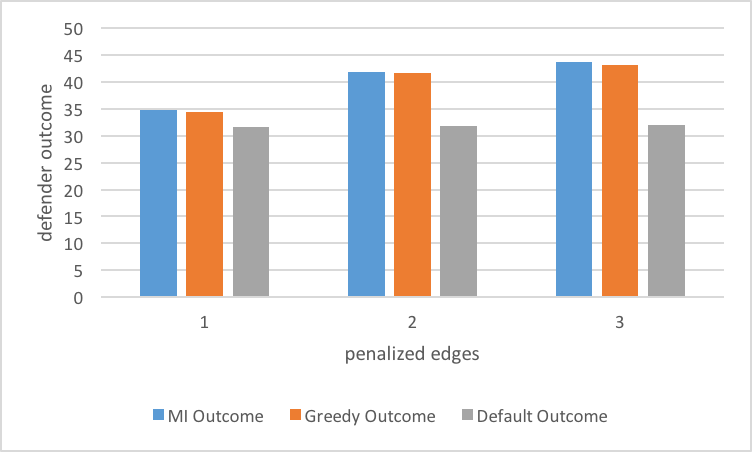
\includegraphics[width=\linewidth]{6}
\caption{Average outcome given penalized edges.}
\label{fig:sol_bar}
\end{minipage}
\end{center}
\end{figure}

\begin{figure}[!ht]
\begin{center}	
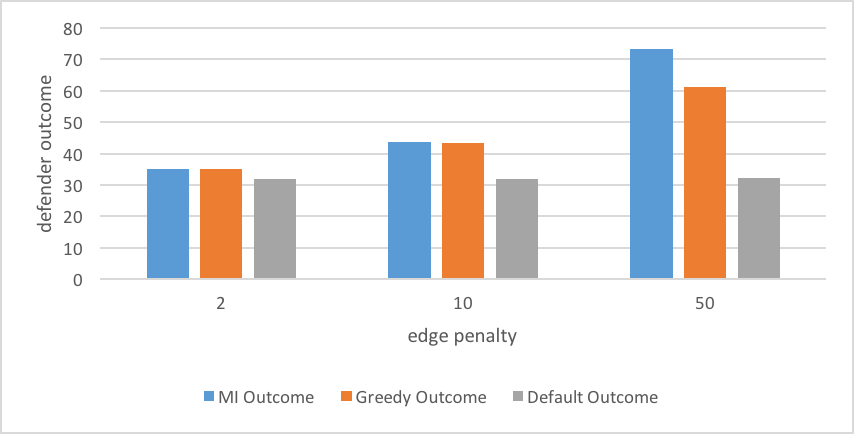
\includegraphics[scale=0.45]{7}
\caption{Average outcome given penalty value.}
\label{fig:sol_ep}
\end{center}
\end{figure}

\subsubsection{Various Number of Barriers/Blocks}
In this set of experiments, we want to investigate 
the effect of different number of barriers (i.e., $K$) 
to the running time (Figure \ref{fig:rt_target}) 
and solution quality (Figure \ref{fig:sol_target}) of our algorithms 
in the GTGRD models.  
The results are averaged over 1000 simulations of 6 by 6 grids. 


%Results in \textbf{Fig. 8} and \textbf{Fig. 9} were averaged over 1000 grids, each with a width and height of 6 nodes. 
%The defenders reward for correctly guessing the adversary's intended target $q$ was set to 10. 
%The attacker penalty value for crossing an edge penalized by the observer was set to 10. 
It turns out that as we increase the number of barriers, 
the running times of our greedy heuristic are longer than 
the MIP as shown in Figure \ref{fig:rt_bar}. 
Nonetheless, as in the earlier experiments, 
both algorithms have similar solution quality. 


\subsubsection{Various Edge Penalties}
Finally, consider the effect of different edge penalties 
to the solution quality of our greedy heuristic. 
The results are averaged over 1000 simulations of 6 by 6 grids. 
As indicated in Figure \ref{fig:sol_ep}, 
the solution gap between the MIP and greedy heuristic 
as we increase the edge penalty. 

%Results in \textbf{Fig. 10} were averaged over 1000 grids, each with a width and height of 6 nodes. 
%The defenders reward for correctly guessing the adversary's intended target $q$ was set to 10. 
%Each game, the observer was permitted to penalize 2 edges.


\nocite{Dijkstra80}
\nocite{plop03-paper}
